% this file is called up by thesis.tex
% content in this file will be fed into the main document

\chapter{Evaluation}\label{ch:evaluation} % top level followed by section, subsection


% ----------------------- paths to graphics ------------------------

% change according to folder and file names
\ifpdf
    \graphicspath{{figures/PNG}}
\else
    \graphicspath{{7/figures/EPS/}{7/figures/}}
\fi


% ----------------------- contents from here ------------------------
% 
In this section, the experimental results are presented.
%First a baseline of RDMA performance on DAS is given.
%This will be used to compare a KV store use case to maximum performance that can be achieved on DAS.
The RDMA transportation types are compared within and against the baseline TCP implementation.
Throughput and latency are mainly used to analysis the multicore scalability of these transportation types; with increasing number of clients, and therefore threads.
For latency three figures have been used to evaluate: average latency, boxplot without outliers, and cumulative distribution function (CDF).
The same raw data is used for both measurements, thus can be compared alongside each other.

The two designs are analyzed, with and without blocking for completion event.
For TCP the same data has been used for evaluation of both designs, as this is used as baseline.

In short, the results show:
\begin{itemize}
    \item Without blocking, throughput reaches an peak, with all transportation types, at roughly 32 clients.
    UC performs best, with a maximum throughput of 370185 ops/sec at 33 clients.
    Further details are given in section \ref{sec:throughput-analysis}.
    \item With blocking, throughput reaches an equilibrium up to 70 clients.
    UC, again, performance best, stabilizing at roughly x ops/sec.
    \item Latency increases across all transportation types, with increased number of clients, and both with and without blocking.
    Results are inversely comparable to throughput, again with UC performing best.
    Without blocking: UC has a average latency of roughly 49.2 $\mu$sec at 32 clients and 179.7 $\mu$sec at 60 clients.
    The spread also increases: standard deviation ranges from 46.6 $\mu$sec at 32 clients, to 1628.2 $\mu$sec at 60 clients.
    UC also performance best due to the stable 95th persentile, which is 110 $\mu$sec for both 32 and 60 clients.
    \item
    With blocking: UD has a average latency of roughly x $\mu$sec at 32 clients and x $\mu$sec at 60 clients.
    The spread also increases: inner quartile range ranges from x $\mu$sec at y clients, to x $\mu$sec at y clients.

    Section \ref{sec:latency:analysis} delves deeper.
\end{itemize}

To recall the benchmarking setup:
Ten million KV-store operations are divided equally between \textit{n}-clients.

\section{Throughput analysis}\label{sec:throughput-analysis}
To compare the overall throughput between TCP, RC, UC, and UD with up to 70 clients.
With non-blocking design, peak throughput performance is realised at roughly 32 clients.
This can be seen in figure \ref{fig:throughput-30}.
For RC, maximum throughput is roughly 247782 ops/sec at 32 clients.
While for UC, maximum throughput is roughly 370185 ops/sec at 33 clients, and for UD this is at roughly 357019 ops/sec at 31 clients.
The maximum throughput TCP achieves in this number of clients range, is 206750 ops/sec at 33 clients.
For RC, UC, and UD this is a percentage increase over TCP of: 19.85\%, 79.05\%, and 72.68\%.
However, after 32 clients, throughput has a sharp decline, with RC failing to connect properly above 60 clients, resulting in incomplete data at these points.
\begin{figure}
    \centering
    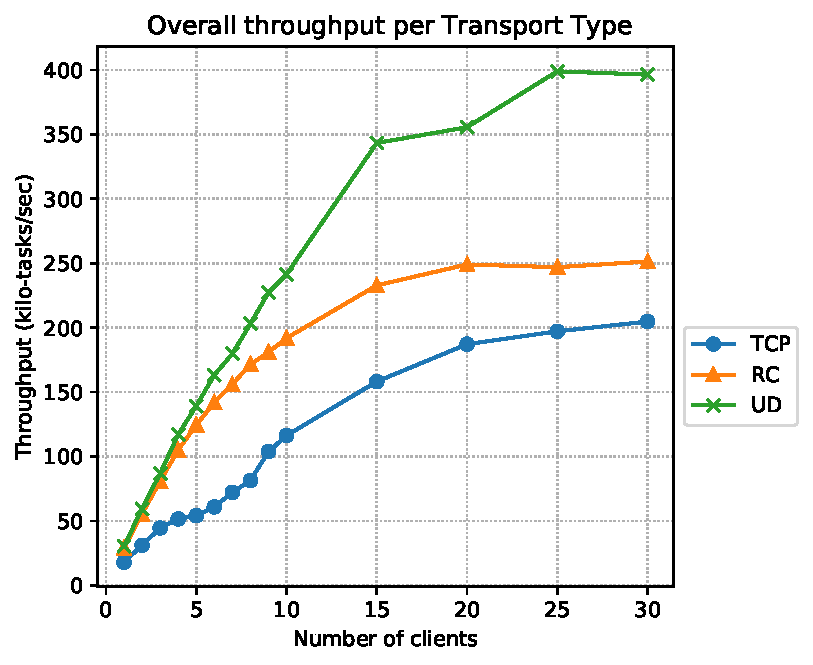
\includegraphics[height=8cm]{figures/PDF/Throughput_30}
    \caption{Throughput of clients executing 10 million operations}
    \label{fig:throughput-30}
\end{figure}

\subsection{Scalability rate}\label{subsec:scalability-rate}
Multicore scalability of all RDMA transportation types, without blocking, is poor.
Up to roughly 15 clients, throughput performance increases at a linear rate.
For TCP, there is an average increase of 10246 ops/sec per additional client.
For the RDMA transport types, for RC this is 16726 ops/sec per additional client, 21462 ops/sec for UC, and 21067 ops/sec for UD.
This shows that unreliable transport types, UC and UD, scale better per additional client and worker thread, compared to RC and TCP.
However, after 15 threads, performance begins to plateau for all transportation types and TCP, showing that the used KV-store is CPU bound.
This is due to the pthread locking, used to provide isolation with concurrent threads operating on the KV-store.

After 32 clients and worker threads, multicore performance weakens, and dropping in performance.
This is due to the non-blocked design, and 32 physical threads being the maximum on a single DAS-5 node.
Without this blocking or scheduling, threads take CPU cycles while polling on the receive queue.
With only a limited number of CPU cycles, this is not used efficiently, resulting in drop in performance for all worker threads.


\begin{table}
    \begin{tabular}{ccccc}
        Clients & TCP & RC & UC & UD \\
        1 & & & & \\
        2 & 6531.571861 & 24686.53216 & 24638.92191 & 26502.60875 \\
        3 & 13594.18984 & 23770.88044 & 24785.06225 & 28301.22973 \\
        4 & 4297.07597 & 24568.10076 & 27795.82235 & 23489.22267 \\
        5 & 7363.59922 & 17665.61705 & 19850.77766 & 22090.10711 \\
        6 & 6521.771444 & 16064.3204 & 20579.02917 & 24167.81283 \\
        7 & 11672.14625 & 13975.27874 & 21439.07072 & 16246.34785 \\
        8 & 18989.11049 & 14401.88884 & 17510.50509 & 14201.32075 \\
        9 & 12033.20216 & 4957.154159 & 17930.69447 & 21432.34552 \\
        10 & 11858.04359 & 18916.31359 & 20129.9112 & 17827.70575 \\
        15 & 9603.176325 & 8252.113695 & 19962.02981 & 16410.46889 \\
    \end{tabular}
    \caption{Throughput increase per additional client}
    \label{tab:throughput_add_client}
\end{table}

%\subsection{Fairness between clients}
%TODO GENERATE GRAPH FOR THIS

\section{Latency analysis}\label{sec:latency:analysis}
An important factor to KV-store is their quick response time.
Latency should ideally scale similarly, preferably better, than throughput, such that with an increased number of clients, latency changes are unnoticed to the clients.
RDMA offers fast response time due to the lack of CPU and kernel involvement.
This can be seen in \ref{fig:rc_latency_30}, where RDMA transportation types perform better than TCP up to 55 clients, after which UD performs worse, and RC following this trend.

\begin{figure}
    \centering
    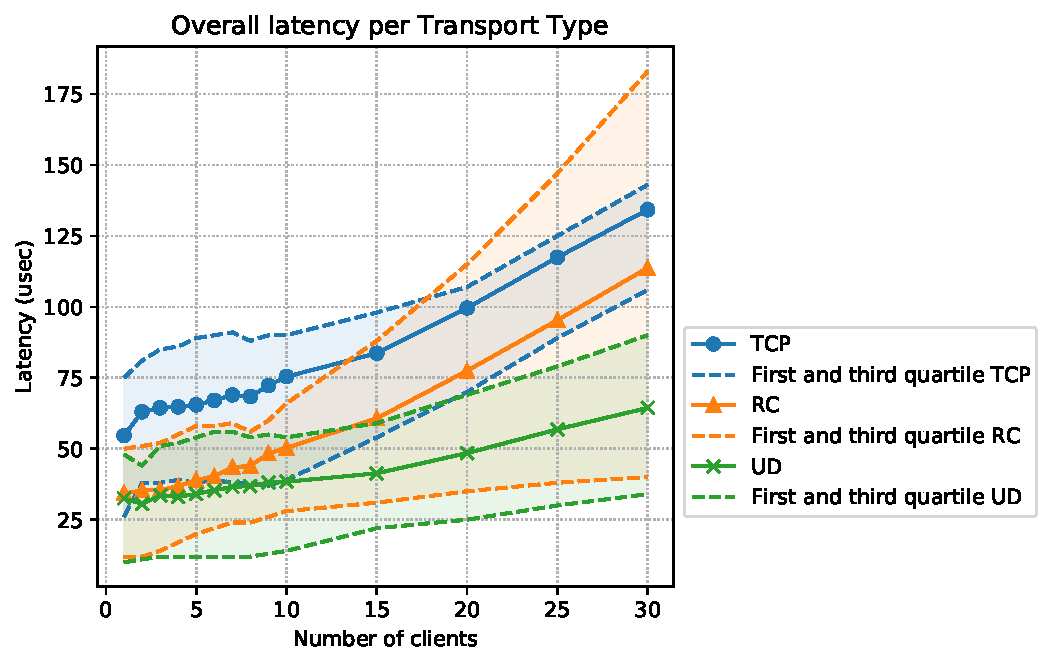
\includegraphics[width=\columnwidth]{figures/PDF/Latency_avg_30}
    \caption{Latency of clients executing 10 million operations}
    \label{fig:latency-30}
\end{figure}

At roughly 32 clients, relative performance is similar to throughput as seen in figure \ref{fig:throughput-30}.
Results show that TCP has an average latency of 138.0 $\mu$sec at 32 clients.
RC has an average latency of 115.1 $\mu$sec, a 16.61\% improvement relative to TCP.
UC performs best at 32 clients, with an average latency of 49.24 $\mu$sec, which is an 64.33\% improvement over TCP.
Finally, UD has an average latency of 65.5 $\mu$sec, which is an improvement of 52.5\% over TCP.

It can also be observed that latency scales proportional with the number of clients for TCP, while this is only the case for RDMA up to roughly 32 clients.
The average rate of change for TCP, RC, UC, and UD up to 32 clients is: 2.31 $\mu$sec, 2.00 $\mu$sec, 0.37 $\mu$sec, and 0.72 $\mu$sec.
This shows that UC scales favorably up to 32 clients, closely followed by UD.
After 32 clients, RDMA transportation types scale worse, with UD surpassing TCP's average latency at 60 clients.
RC is trending towards surpassing TCP after 60 clients, however, this data could not be collected reliably.
Lastly, UC still performs favorably compared to TCP at 70 clients, however, relative performance is now at 21.98\%.





The latency between protocols is an inverse reflection of the throughput graph, scaling and overall performance.
Similarly, TCP performed worst, with an average latency of 134.2 $\mu$sec at 30 clients.
RC hits an average of 113.7 $\mu$sec, also at 30 clients.
UD again performing best, reaching 64.4 $\mu$sec on average.

Single client performance is lacking with HERD\cite{kalia2014using} and FaSST\cite{kalia2016fasst}, and from what should be theoretically possible, being in the order of sub-10 $\mu$sec latency.
This could be due to lock contention with shared QP queues, in the case of UD, and/or poor performance of KV store.
A further examination of this could support this.

Similarly to throughput, UD scales relatively well, while RC and TCP scale linearly.
A near uniform latency for the first 15 clients, afterwards a gradual slope, compared to TCP and RC.





\subsection{Variation from average}
Consistent latency is important for clients, such that performance is predictable.
Therefore, a box plot and CDF graph is used to examine the spread of latency at three points: 5 clients, 32 clients and 60 clients.
Additionally, the median, innerquartile range, 95th and 99th percentile, and standard deviation, is used to examine the spread numerically.
This numeric data can be found in table \ref{tab:num_stats}.
The complete table, with number of clients up to 70, can be found in table INSERT TABLE in the appendix.
\begin{table}
    \subtable[TCP] {
        \centering
        \begin{tabular}{rrrrrr}
            \toprule
            \textbf{Clients} & \textbf{Median} & \textbf{IQR} & \textbf{95th percentile} & \textbf{99th percentile} & \textbf{Standard deviation} \\
            \midrule
            5 & 62 & 55 & 126 & 152 & 33.50 \\
            32 & 129 & 40 & 192 & 233 & 268.86 \\
            60 & 238 & 65 & 318 & 368 & 275.85 \\
            \bottomrule
        \end{tabular}
        \label{tab:num_stats_tcp}
    }

    \subtable[RC] {
        \centering
        \begin{tabular}{rrrrrr}
            \toprule
            \textbf{Clients} & \textbf{Median} & \textbf{IQR} & \textbf{95th percentile} & \textbf{99th percentile} & \textbf{Standard deviation} \\
            \midrule
            5 & 31 & 43 & 88 & 99 & 29.33 \\
            32 & 112 & 149 & 227 & 231 & 83.10 \\
            60 & 48 & 56 & 120 & 7852.41 & 1662.83 \\
            \bottomrule
        \end{tabular}
        \label{tab:num_stats_rc}
    }

    \subtable[UC] {
        \centering
        \begin{tabular}{rrrrrr}
            \toprule
            \textbf{Clients} & \textbf{Median} & \textbf{IQR} & \textbf{95th percentile} & \textbf{99th percentile} & \textbf{Standard deviation} \\
            \midrule
            5 & 29 & 49 & 84 & 95 & 29.26 \\
            32 & 39 & 70 & 110 & 122 & 46.59 \\
            60 & 35 & 56 & 110 & 1296 & 1629.16 \\
            \bottomrule
        \end{tabular}
        \label{tab:num_stats_uc}
    }

    \subtable[UD] {
        \centering
        \begin{tabular}{rrrrrr}
            \toprule
            \textbf{Clients} & \textbf{Median} & \textbf{IQR} & \textbf{95th percentile} & \textbf{99th percentile} & \textbf{Standard deviation} \\
            \midrule
            5 & 29 & 46 & 84 & 95 & 30.45 \\
            32 & 57 & 64 & 126 & 146 & 65.59 \\
            60 & 54 & 65 & 143 & 9036 & 1693.72 \\
            \bottomrule
        \end{tabular}
        \label{tab:num_stats_ud}
    }

    \caption{Numeric statistic latency. All statistical values have unit $\mu$sec. IRQ is short for innerquartile range}
    \label{tab:num_stats}
\end{table}

From this it can be observed that from these three points, standard deviation increases as number of clients increase.
With RDMA, there is a signficant increase in variation after 32 clients.
The median latency and 95th percentile of UC and UD remains similiar between 32 and 60 clients, however the outliers or 99th percentile, increase significantly.
This is further supported by the CDF figure of 32 clients INSERT FIGURE REF and 60 clients INSERT FIGURE REF.
In these figures, 80\% of the data is near 100 $\mu$sec and 90 $\mu$sec, for UD and UC respectively, deviating slightly between 32 and 60 clients.
However, the top 1\% of the data is not below the 500 $\mu$sec shown for 60 clients, while this is the case for 32 clients.
These outliers are caused by polling and concurrent number of threads, which exceed the number of physical threads.
With high CPU usage, the time until a new request is seen and can be processed, increases, causing a delay for the client.
These outliers can be also seen to cause the loss in throughput performance.

It can also be observed that RC suffers from a peak spread around 32 clients, which afterwards falls back down.
Innerquartile range reaches a peak of 149 $\mu$sec at 32 clients, with a median of 112 $\mu$sec.
It is unclear what causes this, however should be considered when reaching maximum number of physical threads.



In figure \ref{fig:latency-30} the variation is given in form of first and third quartile.
It can be seen that TCP and UD have a constant, a small, variation.
TCP is skewed towards higher latencies at 30 clients, while UD, and RC, stay normally distributed throughout.
RC has a rapidly increasing variation, which is concerning for scalability and consistency.
As number of clients increases, the realised latency could vary drastically between tasks.
These issues could possibly be due to context switching, more in subsection \ref{subsec:rdma-multiple-qp's-causing-cache-misses-and-context-switching} below.

\subsection{All 30 clients and per operation latency}\label{subsec:all-30-clients-and-per-operation-latency}

\begin{figure}
    \centering
    \subfigure[TCP] {
        \centering
        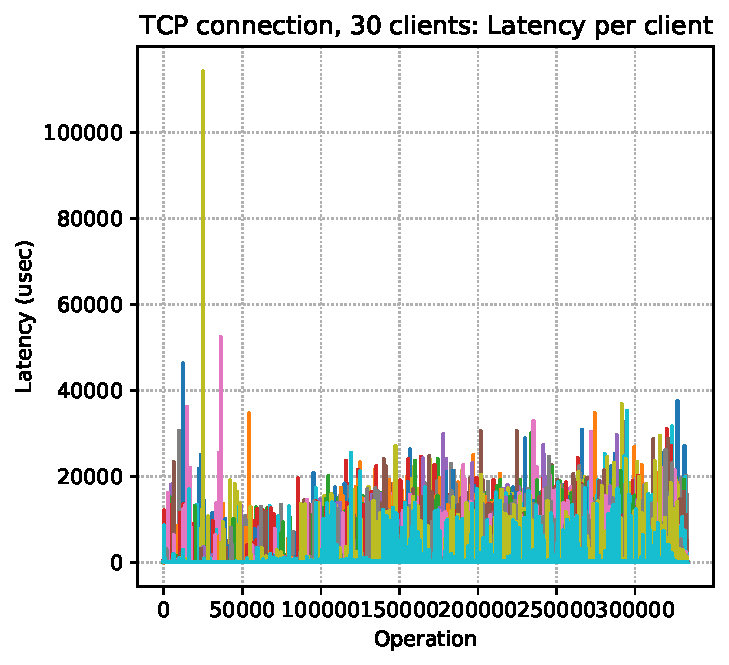
\includegraphics[width=0.47\columnwidth]{figures/PDF/TCP_Latency_30}
        \label{fig:tcp_latency_30}
    }
    \subfigure[RC] {
        \centering
        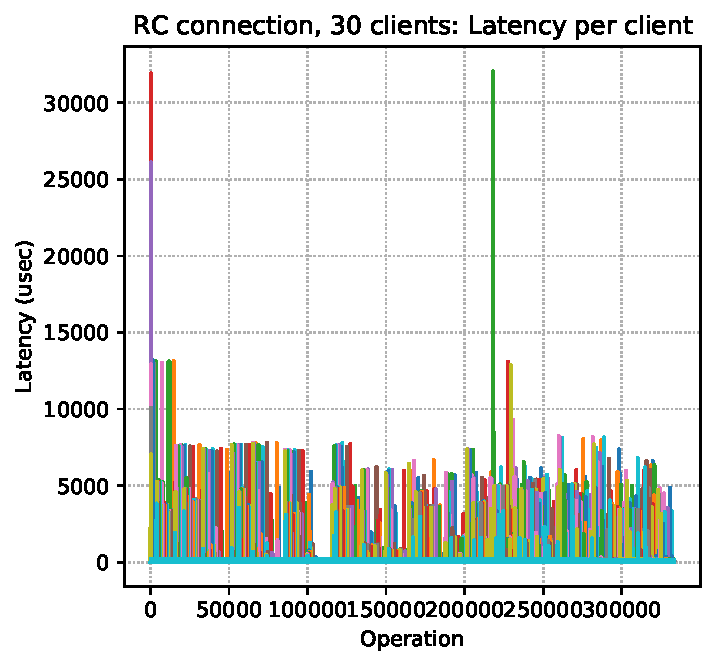
\includegraphics[width=0.47\columnwidth]{figures/PDF/RC_Latency_30}
        \label{fig:rc_latency_30}
    }
    \subfigure[UD] {
        \centering
        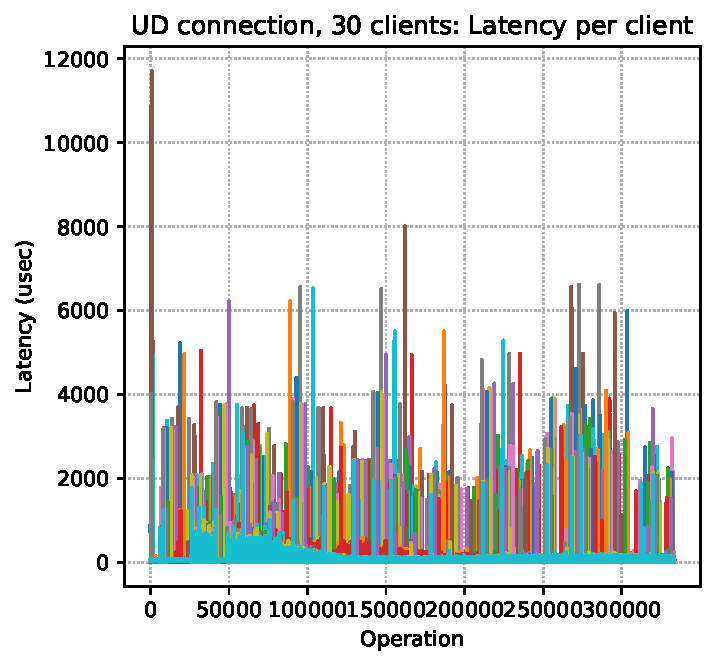
\includegraphics[width=0.47\columnwidth]{figures/PDF/UD_Latency_30}
        \label{fig:ud_latency_30}
    }
    \caption{Structure for response with accommodated response codes}
    \label{fig:latencies_30}
\end{figure}


Figure \ref{fig:latencies_30} delves deeper into the details of the latency outliers that are present.
Note on the scale, not similar between protocols, and compared to figure \ref{fig:latency-30}.
These outliers are the extreme outliers, not displayed in figure \ref{fig:rc_latency_30}.
TCP and RC see spikes up to 114185 $\mu$sec, or 114.2ms, and 32046 $\mu$sec, or 32.05ms.
UD on the other only spikes to a maximum of 11702 $\mu$sec, or 11.7ms.
These outliers have a significant impact on the realised performance.
In the case of TCP and UD, these seem to occur at random.
For RC this does not seem to be the case, which suggests a systematic error is at cause.

\subsection{RDMA multiple QP's causing cache misses and context switching}\label{subsec:rdma-multiple-qp's-causing-cache-misses-and-context-switching}
In section \ref{subsec:transportation-types} the issue with holding multiple QP's within the RNIC, has been discussed.
The RNIC needs to perform context switching when changing QP.
As the number of QP's increase, the number of context switches needed increases.
Along this, the chance of cache misses are also increased.
This decreases the performance, with increased latency, and in throughput as shown here.
With context switching, a large delay occurs, and harms the performance per client, but also of the overall network.
For this reason, for large number of clients, a one-to-one QP, such as RC and UC, is not advisable.

\subsubsection{Cache misses as increased variation for RC}
Furthermore, cache misses occur more often at the starting phase of KV store operations, as can be seen in section \ref{fig:rc_latency_30} above.
RC has consistently higher latency (0.75ms) for some clients at the start.
Initially it was thought to be retransmissions, however for this was set to 67.1ms.
Since this only occurs to some clients, and not all, this could be a result from the aforementioned context switching and RNIC cache misses.
At the start of operations, worker threads are operating in sync.
This would result in RNIC processing multiple WR's concurrently.
Some QP's will be cached and experience little cache misses throughout the starting phase, while others would encounter cache misses repeatedly.
Once threads are out of sync and KV store operation latency increases (due to the increasing size of the hash table), the cache misses will occur for all QP's.
This can be seen in figure \ref{fig:rc_latency_30}, as the latency in the final phase is randomized and less constant, compared to the starting phase.

With cache misses, latency per client varies, as some QP's would require further lookup after cache miss.
This effect can be seen in figure \ref{fig:latency-30}, as increasing number of clients, and therefore QP's, increases the variation dramatically.
Further investigation into cache misses would support these claims, this has not been done for this thesis.

% ---------------------------------------------------------------------------
% ----------------------- end of thesis sub-document ------------------------
% ---------------------------------------------------------------------------